\chapter{Dimensionering af stålprofiler}

Figur \ref{fig:hej} viser de nye byggefelter inden for henholdsvis delområde A og delområde B til Strøybergs Palæ (\citep{lokalplan}, s. 16). Denne rapport fokuserer på byggefeltet inden for delområde B, hvor ny bebyggelse, ifølge lokalplan 1-1-107, må opføres i 3 etager samt en tagetage og med en kælder maksimalt 2 m over terræn. Ved opførsel af ny bebyggelse i delområde B, skal to nuværende mindre bygninger fjernes. 

\begin{figure}[htbp]
	\centering
	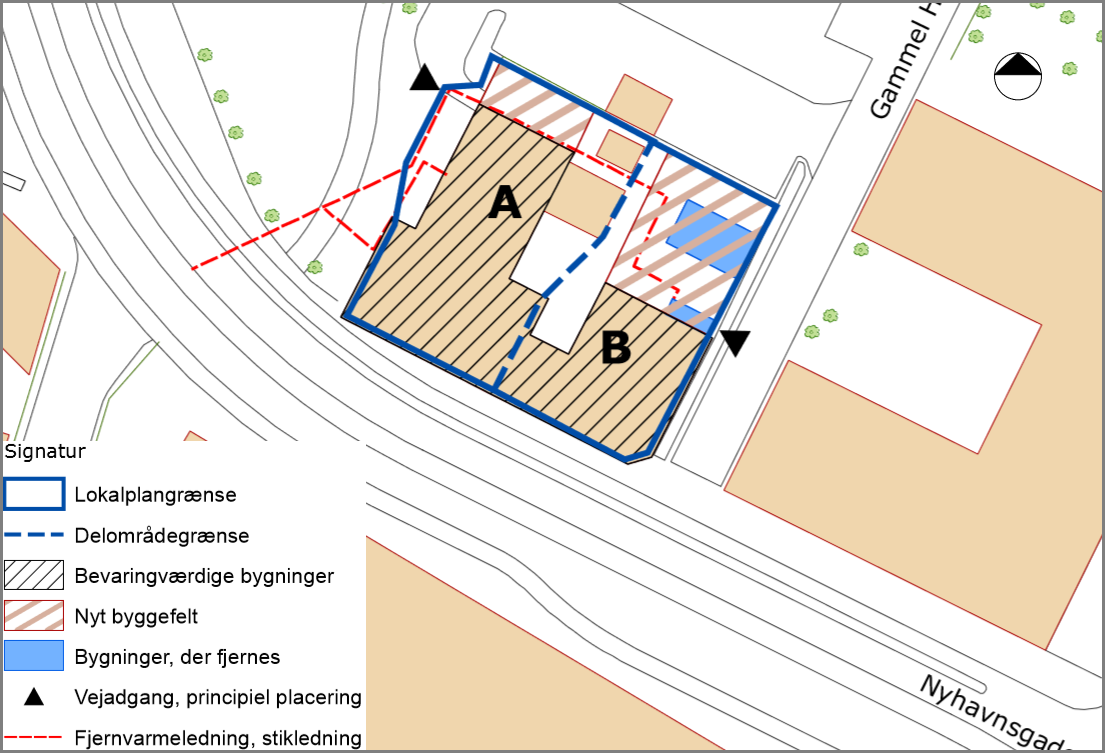
\includegraphics[width=0.8\textwidth]{billeder/signatur.png}
	\caption{Lokalplan 1-1-107, delområde A og B \citep{lokalplan[ bilag 2, s. 35]}}
	\label{fig:hej}
\end{figure}

Med udgangspunkt i lokalplan 1-1-107 har bygningen fået de størrelser og dimensioner, som ses på Figur \ref{fig:farvel}.
\newline \indent{     }  Tilbygningen bliver $12,\!5$ meter lang og 12 meter bred i henhold til den eksisterende bygningsbredde. Kælderen har en højde på i alt $3,\!25$ m, hvor $1,\!25$ m ligger over terræn. Stueetagen, 1. sal og 2. sal har hver især en højde på $4,\!9$ m og tagetagen har en højde på 3 meter med en hældning på $26,\!6$ grader. I alt er tilbygningen 19 m høj over terræn.

\begin{figure}[htbp]
	\centering
	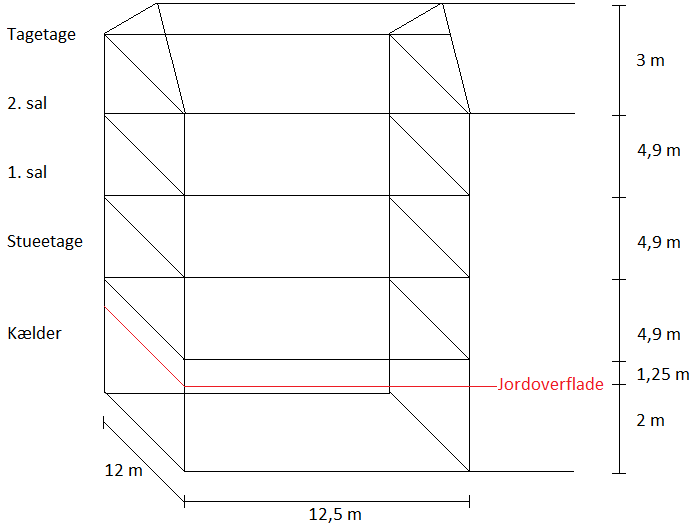
\includegraphics[width=0.7\textwidth]{billeder/tilbygning2.png}
	\caption{Tilbygningens dimensioner}
	\label{fig:farvel}
\end{figure}

For at kunne beregne de laster som påvirker tilbygningen, er der opstillet nedenstående statisk system for bygningen. Systemet er opstillet som en bjælkekonstruktion.
\newline
\newline
Beregningerne opdeles for to gavle og to facader. Det antages at gavlene hver er 12 m lang og 16 m høj, eksklusiv en gavltrekant med en højde på 3 m, og har 9 vinduer med dimensionerne; $0,\!95$ m bred og $1,\!5$ m høj.
\newline
\newline
De to facader er $12,\!5$ m lang og 16 m høj. Den har 11 vinduer, med samme mål som for vinduerne på gavlene, og en dør, som er $1,\!5$ m bred og $2,\!1$ m høj.
\newline
\newline
For at kunne beregne de laster, som påvirker tilbygningen, er der opstillet et statisk system for tilbygningen. Systemet er opstillet som en bjælkekonstruktion og indeholder tre rammekonstruktioner som vist på Figur \ref{fig:system}.

\begin{figure}[htbp]
	\centering
	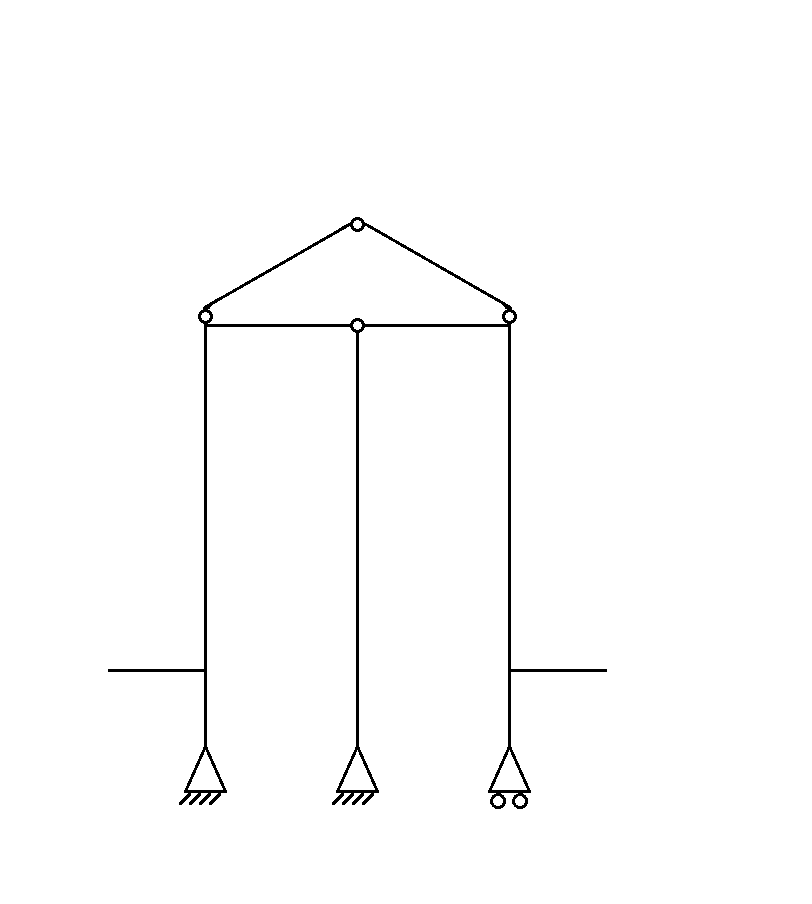
\includegraphics[width=0.3\textwidth]{billeder/del1statiskesystem.png}
	\caption{Statiske system}
	\label{fig:system}
\end{figure}

På disse rammekonstruktioner vil etagedækkene virke som en belastning, i stedet for at virke som en del af konstruktion. Dette er muligt, da der kan opsættes en samling mellem etagedækkene og stålkonstruktion, som ses på Figur \ref{fig:etage}.

\begin{figure}[htbp]
	\centering
	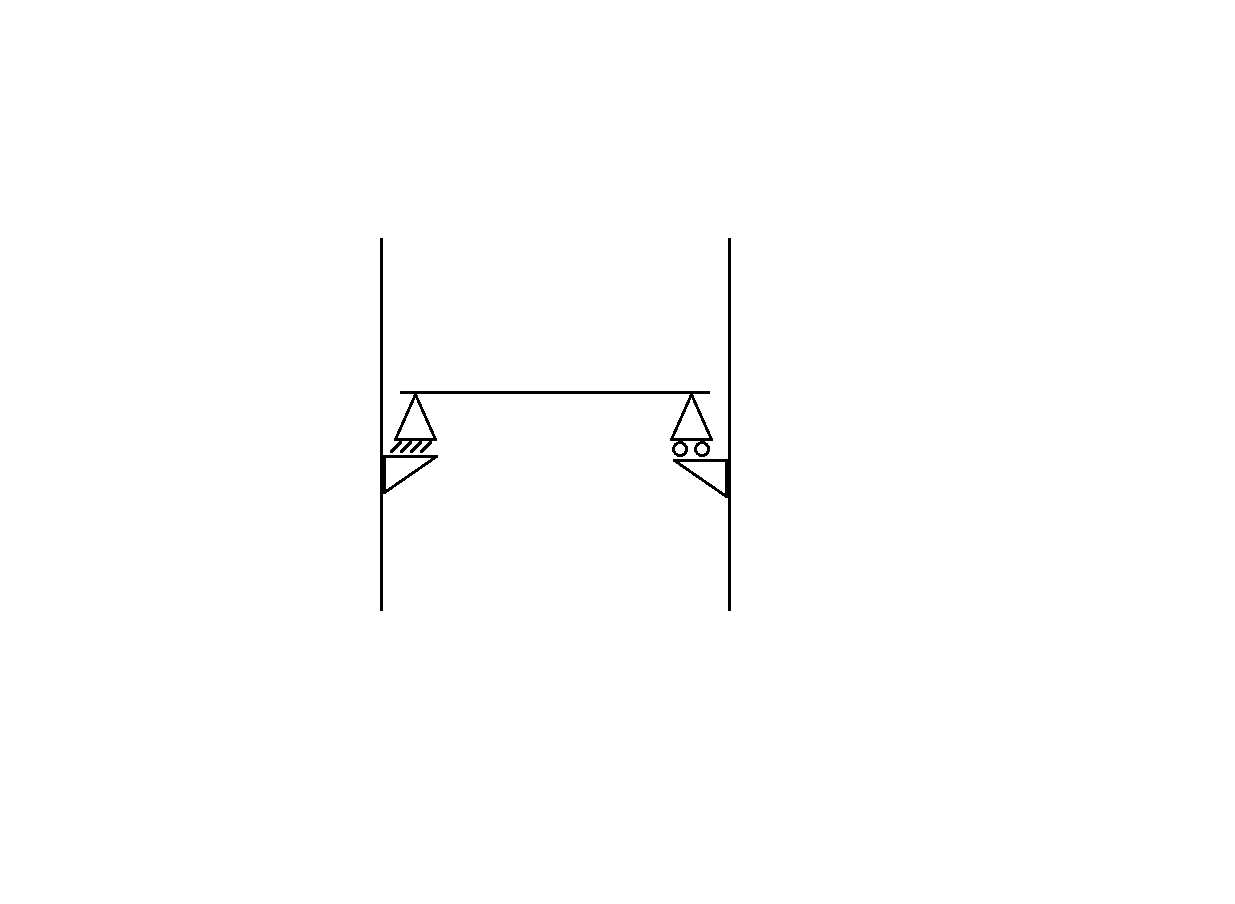
\includegraphics[width=0.2\textwidth]{billeder/etageovergang.png}
	\caption{Etageovergang på tilbygningen}
	\label{fig:etage}
\end{figure}

Med denne opstilling kan reaktionerne beregnes og der ud fra finde belastningen, som vil komme på funderingen, men først skal lasterne beregnes.

\section{Laster}
Tilbygningen til Strøybergs Palæ vil blive udsat for en række forskellige laster, både permanente- og variable laster, hvilke vil blive beregnet i dette afsnit således, at der senere hen kan opstilles lastkombinationer, regnes reaktionskræfter, snitkræfter, spændinger samt brudgrænse- og anvendelsesgrænsetilstande.

\subsection{Permanente laster}
Egenlaster er permanente laster. For tilbygningen til Strøybergs Palæ beregnes disse laster gennem de gjorte antagelser samt de givne mål, som er illustreret på Figur \ref{fig:farvel}.
\newline
\newline
\textbf{last fra tagsystem}
\newline
Det antages at taget, som benyttes, er et mellemtungt tag, som har værdien $600 \frac{N}{m^2}$ \citep{tag}, og det er et sadeltag med teglsten. Der er derfor fundet en middelværdi for lasten fra taget til systemet. 
\newline
\newline
Tagets areal bestemmes ud fra Figur \ref{fig:tagetage}:
\begin{center}
	$6,\!7 m\cdot 12,\!5 m \cdot 2=167,\!500 m^2$
\end{center}

Arealet ganges med værdien for mellemtungt tag:
\begin{center}
	$167,\!500 m^2\cdot 600 \frac{N}{m^2}=100,\!500 kN$
\end{center}

\textbf{Last fra væg}
\newline
\newline
\underline{Facade}
\newline
Facaderne antages for at være ens samt indeholde lige mange vinduer og døre. Der antages at være 11 vinduer og én dør pr. facade \citep{gammellokalplan}, hvilket illustreres på Figur \ref{fig:facade}.

\begin{figure}[htbp]
	\centering
	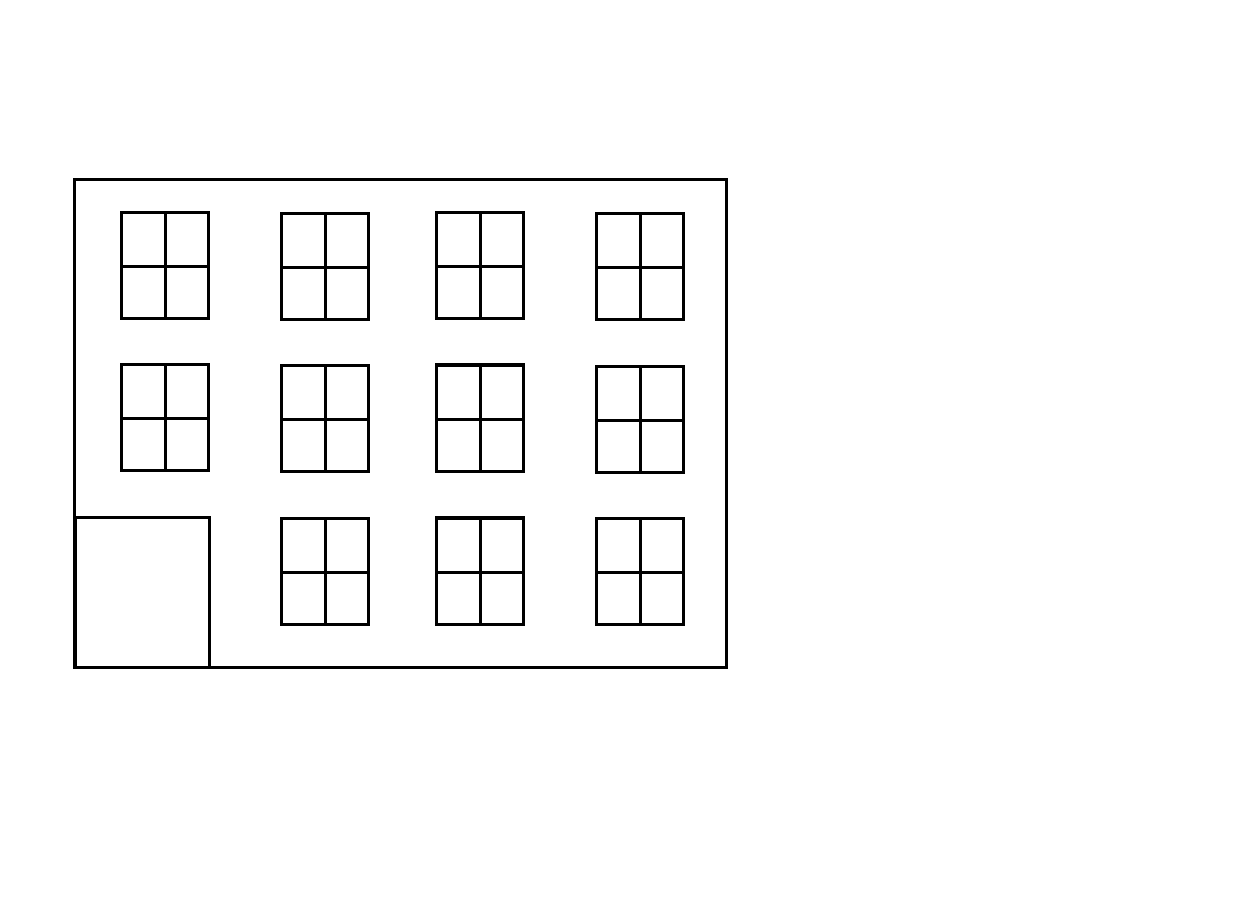
\includegraphics[width=0.8\textwidth]{billeder/facadenord.png}
	\caption{Facaden på øst- og vestsiden}
	\label{fig:facade}
\end{figure}

\indent{     }  Ét vindue antages til være $0,\!95$ m bred og $1,\!5$ m høj. Døren antages at være $1,\!5$ m bred og $2,\!1$ m høj. Arealet for én facade bestemmes til:
\begin{center}
	$12,\!5 m\cdot 16,\!0 m - (1,\!5 m\cdot0,\!95 m\cdot11 + 1,\!5 m\cdot 2,\!1 m)=181,\!175 m^2$
\end{center}

Til beregning af væggens egenlast vides det, at der skal påregnes en indervæg og et isoleringslag, mens den ydervæggen ikke er en del af det statiske system og dermed ikke skal medregnes.
\newline \indent{     }  En typisk indervæg er typisk 130 mm tyk \citep{indervaeg}, og det antages, at denne værdi benyttes til tilbygningen af Strøybergs Palæ. Dermed kan værdien for indervæggen af facaden nu bestemmes ved at gange facadens areal uden viduer og dør med tykkelsen, hvorefter denne værdi ganges med densiteten for mursten \citep{murstendensitet}, hvilket er $1500,\!0 \frac{kg}{m^3}$:
\begin{center}
	$181,\!175 m^2\cdot 130 mm\cdot 1500,\!0 \frac{kg}{m^3}\cdot 9,\!82 \frac{m}{s^2}=35329,\!125 kg$
\end{center}

Denne værdi omregnes til $N$ ved at gange med tyngdeaccelerationen:
\begin{center}
	$35329,\!125 kg\cdot 9,\!82 \frac{m}{s^2}=346,\!932 kN$
\end{center}

I og med facaderne er identiske ganges de $346,\!932 kN$ med 2:
\begin{center}
	$346,\!932 kN\cdot 2=693,\!864 kN$
\end{center}

Isoleringslaget regnes til at være 100 mm tyk \citep{isolering}, og det antages, at typen af isolering har densiteten $30 \frac{kg}{m^3}$ \citep{densitet}.
\newline \indent{     }  Facadens areal uden vinduer og dør med tykkelsen, hvorefter denne værdi ganges med densiteten for isoleringen:
\begin{center}
	$181,\!175 m^2\cdot 0,1 \cdot 30 \frac{kg}{m^3}\cdot 9,\!82 \frac{m}{s^2}=5,\!337 kN$
\end{center}

I og med facaderne er identiske ganges de $5,\!337 kN$ med 2:
\begin{center}
	$5,\!337 kN\cdot 2=10,\!675 kN$
\end{center}

\underline{Gavl}
\newline
Da den ene gavl ligger op ad den nuværende bygning, vil der ikke være vinduer på denne gavl, mens der antages at være 9 vinduer, identiske med dem for facaden, for gavlen, der ikke ligger op ad den nuværende bygning, som kan ses på Figur \ref{fig:gavl}.

\begin{figure}[htbp]
	\centering
	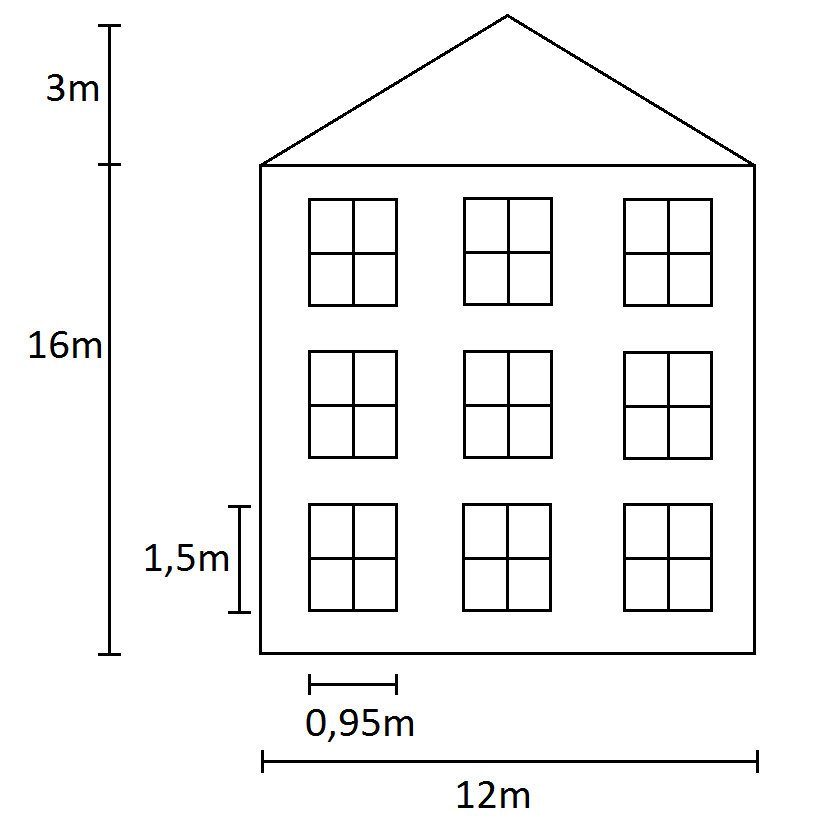
\includegraphics[width=0.6\textwidth]{billeder/facadevestellerost.png}
	\caption{Dimensioner for tagetagen}
	\label{fig:gavl}
\end{figure}

Til forskel for facadens areal, har gavlene også arealet for tagetagen, som har dimensionerne der ses på Figur \ref{fig:tagetage}. Arealet for facaden der ikke ligger op ad den nuværende bygning bestemmes dermed til:
\begin{center}
	$12 m\cdot 16 m + 3 m\cdot 12 m \cdot 0,\!5 - 1,\!5 m\cdot 0,\!95 m \cdot 9=197,\!175 m^2$
\end{center}

\begin{figure}[htbp]
	\centering
	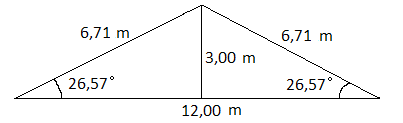
\includegraphics[width=0.7\textwidth]{billeder/Tagmedvinkel.png}
	\caption{Dimensioner for tagetagen}
	\label{fig:tagetage}
\end{figure}

Ligesom for facaderne skal der også påregnes en indervæg og et isoleringslag for gavlen, og det antages at der anvendes den samme tykkelse og densitet for indervæg og isolering.
\newline
\newline
Værdien for indervæggen bestemmes til:
\begin{center}
	$197,\!175 m^2\cdot 130 mm\cdot 1500,\!0 \frac{kg}{m^3}\cdot 9,\!82 \frac{m}{s^2}=377,\!570 kN$
\end{center}

Værdien for isolering bestemmes til:
\begin{center}
	$197,\!175 m^2\cdot 100 mm\cdot 30 \frac{kg}{m^3}\cdot 9,\!82 \frac{m}{s^2}=5,\!809 kN$
\end{center}

\textbf{Last fra gulv}
\newline
Det antages at bygnings etager kun består af gulv, dvs. ingen skillevægge, trapper og andre former for genstande, der mindsker mængden af gulv. Derfor er den samlede mængde gulv pr. etage $12,\!5 m\cdot 12,\!0 m=150,\!0 m^2$.
\newline \indent{     }  Fire ud af de fem etager består af bærende gulv, hvor den sidste, kælderetagen, ligger på fundamentet. Et bærende gulv antages at bestå af et armeret betondæk nederst, der oftest er mellem 80 mm og 200 mm tyk. Der antages, at den er 120 mm tyk, hvorpå der ligger bjælker. Bjælkernes opgave er at lede og overføre lasterne ud i understøtning. Derefter vil ligge et undergulv, mellemgulv og til sidst selve gulvbelægningen, og mellem betondækket og undergulvet lægges isoleringen \citep{Gulvopbygning}. 
\newline \indent{     }  Først bestemmes gulvets last for en etage, hvorefter denne ganges denne med fire, da der er fire etager foruden kælderetagen. Betondækkets andel beregnes først, da både længden, bredden og tykkelsen kendes. 
\newline
\newline
Rumfanget af betonen for én etage bestemmes til:
\begin{center}
	$12,\!5 m\cdot 12,\!0 m\cdot 120 mm=18,\!0 m^3$
\end{center}

Rumfanget ganges med betons densitet, som er $2400 \frac{kg}{m^3}$ \citep{betonsdensitet}, hvorefter hvorefter denne værdi ganges med tyngdeaccelerationen, for at få værdien i $kN$, som der ganges med 4 for at få lasten for alle fire etager:
\begin{center}
	$18,\!0 m^3\cdot 2400 \frac{kg}{m^3}\cdot 9,82 \frac{m}{s^2}\cdot 4=1693,440 kN$
\end{center}

Der er behov for bjælker, som hver er $6,\!25$ m lang, da de er halvdelen af tilbygningens længde, $140,\!0$ mm høj og $140,\!0$ mm bred \citep{granse}. Disse anlægges langs med tilbygningen. For at bestemme hvor mange bjælker, der er behov for, divideres længden af tilbygningen med 400 mm, da der skal være 400 mm imellem hver bjælke \citep{Gulvopbygning}. 

\begin{center}
	$\frac{12,\!5 m}{400 mm}=31,\!25$ bjælker
\end{center} 

Da der ikke kan optræde $31,\!25$ bjælker rundes der op til 32 bjælker.
\newline
\newline
Rumfanget af én bjælke, som består af to bjælker med længden $6,\!25$ m, ganges med bjælkens densitet for tørrumvægt af træ \citep{torrumvagt}, hvorefter denne værdi ganges med tyngdeaccelerationen og ganges med 4: 
\begin{center}
	$7,\!840 m^3\cdot 510 \frac{kg}{m^3}\cdot 9,\!82 \frac{m}{s^2}\cdot 4=157,\!057 kN$
\end{center}

Isoleringsarealet for tilbygningen er det samlede gulvareal minus det areal, som bjælkerne ligger på:
\begin{center}
	$150,\! m^2 - (140 mm\cdot 12,\!5 m\cdot 32)=94,\!0 m^2$
\end{center}

Isoleringslaget har samme højde som bjælkerne og har en densitet på $30 \frac{kg}{m^3}$ \citep{densitet}. Dermed kan værdien for isolering bestemmes til:
\begin{center}
	$94,\!0 m^2\cdot 140 mm\cdot 30 \frac{kg}{m^3}\cdot 9,\!82 \frac{m}{s^2}\cdot 4=15,\!508 kN$
\end{center}

Gulvbelægningen antages for at være linoleumsgulv med en højde på $2,\!5 mm$ og en densitet på $2,\!9 \frac{kg}{m^3}$ \citep{linoleum}. 
Dermed kan værdien for linoleumsgulv bestemmes til:
\begin{center}
	$2,\!5 mm\cdot 12,\!5 m\cdot 12,\!0 m\cdot 2,\!9 \frac{kg}{m^3}\cdot 9,\!82 \frac{m}{s^2}\cdot 4=0,\!043 kN$
\end{center}

\textbf{Samlet egenlast eksklusiv tag og stålsystem}
\newline
De tidligere beregnede værdier adderes; 
\begin{center}
	$346,\!932 kN + 346,\!932 kN + 5,\!337 kN + 5,\!337 kN + 377,\!509 kN + 5,\!809 kN + 1693,\!440 kN + 157,\!057 kN + 15,\!508 kN + 0,\!043 kN = 2953,\!904 kN$
\end{center}
Den samlede egenlast deles med 2, da midterrammen optager halvdelen af den beregnede last. 
\begin{center}
	$\frac{2953,904 kN}{2} =  1476,\!952 kN$
\end{center}
Den midterste stang optager $\frac{2}{4}$ af egenlasten, mens de to yderste stænger hver optager $\frac{1}{4}$.

\begin{center}
	$\frac{1476,952 kN}{4} =  369,\!24 kN$
\end{center}

Denne last laves nu om til en linjelast ned langs stængerne, og derfor deles med 18m:
 
\begin{center}
	$\frac{369,24 kN}{18m} =  20,\!51 \frac{kN}{m}$
\end{center}

Den midterste stang optager $\frac{2}{4}$ af egenlasten, mens de to yderste stænger hver optager $\frac{1}{4}$. 
\newline
\newline
\textbf{Egenlast af stålsystemet}
\newline
\underline{egenlast stål i tagsystemet}
\newline
Stålstyrken, som er anvendt, antages at være S235 med profil nr. S450, som har densiteten $g=115\frac{kg}{m}$ \citep{Stabi}. Dette skal ganges med højden af sadeltaget, som er $6,\!7m$.og omregnes efterfølgende til KiloNewton.  
\begin{center}
	$115\frac{kg}{m}\cdot 6,\!7m = 771,\! 42 kg$
	$771,\! 42kg\cdot 9,\! 82\frac{m}{s^2} = 7,\! 5753444 kN$
\end{center}
Denne værdi skal ganges med to, da der går to stålstænger op ved taget:

\begin{center}
$7,\! 58kN \cdot 2 = 15,\! 1506888 kN$
\end{center}

\underline{Stålsystem eksklusiv tag}
\newline
Stålstyrken antages igen at være S235, som har densiteten $g=115\frac{kg}{m}$ \citep{Stabi}. For at finde kraften af en enkelt lodret stang multipliceres denne med højden af bygningen, som er 18 m, inklusiv kælderen.
\begin{center}
	$115\frac{kg}{m}\cdot 18m = 2070 kg$
	$2070 kg \cdot 9,\!82\frac{m}{s^2} = 20,\! 33 kN$
\end{center}

Dette skal omregnes til at blive en linjelast og der divideres derfor med højden igen:

\begin{center}
$\frac{20,\! 33 kN}{18m} = 1,\! 13\frac{kN}{m}$
\end{center}

Det samme skal gøres for at finde kraften for en vandret stang, og densiteten skal her ganges med længden af den vandrette bjælke, som er 6 m.
\begin{center}
	$115\frac{kg}{m}\cdot 6m = 690 kg$
	$690 kg \cdot 9,\!82\frac{m}{s^2} = 6,\!78  kN$
\end{center}

Dette skal omregnes til at blive en linjelast og der divideres derfor med længden af den vandrette stang:
$\frac{6,\! 78 kN}{6m} = 1,\! 13\frac{kN}{m}$
\newline
\newline
\textbf{Opsamling}
\newline
Nu er alle egenlasterne fra taget, etagedækkene samt egenlasten fra stålsystemet fundet. Disse placeres nu i det statiskesytem vidst på figur \ref{fig:dsadsd}

%Ikke det rigtige billede%
\begin{figure}[htbp]
	\centering
	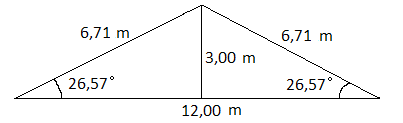
\includegraphics[width=0.7\textwidth]{billeder/Tagmedvinkel.png}
	\caption{Dimensioner for tagetagen}
	\label{fig:tagetage}
\end{figure}

\subsection{Variable laster}
Af variable laster optræder der både snelast, vindlast og nyttelast på bygningen. Disse udregnes efter Dansk Standard Eurocode 1991.

\subsubsection{Snelast}
Til at beregne hvordan snelasten påvirker tilbygningen anvendes den karaktiske snelast og formlen:
\begin{center}
$s=\mu_iC_eC_ts_k$
\end{center}
\begin{itemize}
	\item[-] $s$: karakteristisk snelast
	\item[-] $\mu_i$: formfaktoren for snelasten, som sættes til 0.8 \citep[ tabel 5.2 kapitel 5.3]{EU91}
	\item[-] $C_e$: eksponeringsfaktoren
	\item[-] $C_t$: termisk faktor, som sættes til $1,\!0$ \citep[ kapitel 5.2]{EU91}
	\item[-] $s_k$: karakteristisk terrænværdi, som sættes til $1 \frac{kN}{m^2}$ \citep[ kapitel 4.1]{EU91}
\end{itemize}
Til at bestemme den karakteristiske snelast, beregnes eksponeringsfaktoren $C_e$.
\newline
\newline
Eksponeringsfaktoren, $C_e$, bestemmes ved:
\begin{center}
$C_e=C_{top}C_s$
\end{center}
\begin{itemize}
	\item[-] $C_{top}$: topografi faktor, som sættes til $1,\!0$ \citep[ tabel 5.1 kapitel 5.2]{EU91}
	\item[-] $C_s$: størrelse faktor, som sættes til $1,\!0$ \citep[ kapitel 5.2]{EU91}
\end{itemize}
Eksponeringsfaktoren kan nu bestemmes til:
\begin{center}
$C_e=1,\!0\cdot 1,\!0=1,\!0$
\end{center}
Strøybergs Palæ har et saddeltag, og dermed skal der tages højde for fire lasttilfælde, som ses på Figur \ref{fig:sne}. Derudover ganges snetilfældets værdi med 6,25 m, som er halvdelen af tilbygningens længde, hvilket gøres, da det statiske system er opdelt i tre rammer, for at få værdien ud i $\frac{kN}{m}$.

\begin{figure}[htbp]
	\centering
	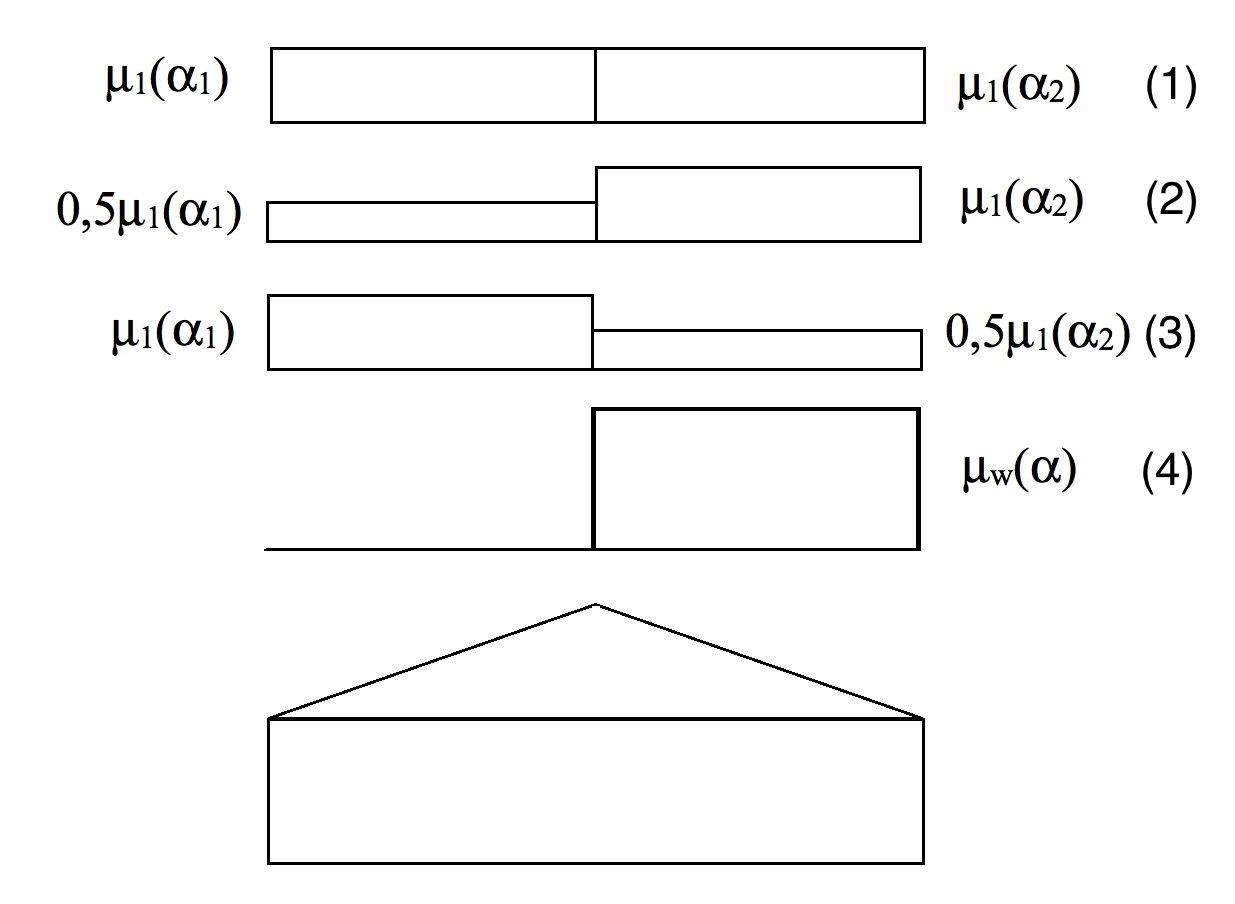
\includegraphics[width=0.6\textwidth]{billeder/snelasttilfaelde.png}
	\caption{Fordeling af sne i de fire tilfælde}
	\label{fig:sne}
\end{figure}

\underline{Snetilfælde 1}
\begin{center}
$s_1=0,\!8\cdot 1.0\cdot 1,\!0\cdot 1 \frac{kN}{m^2}\cdot 6,\!25 m=5,\!0 \frac{kN}{m}$
\end{center}
\underline{Snetilfælde 2 og 3}
\begin{center}
$s_2=\frac{1}{2}\cdot 0,\!8\cdot 1,\!0\cdot 1,\!0\cdot 1 \frac{kN}{m^2}\cdot 6,\!25 m=2,\!5 \frac{kN}{m}$
\end{center}
\underline{Snetilfælde 4}
\begin{center}
	$s_4=\mu_wC_eC_ts_k \frac{kN}{m^2}$
\end{center}
\begin{itemize}
	\item[-] $\mu_w$: formfaktoren, som sættes til $1,\!2$ eftersom $\alpha$ er $26,\!565^{\circ}$ \citep[ kapitel 5.3.3]{EU91}
\end{itemize}
Den karakteristiske snelast for lasttilfælde 4 kan nu bestemmes til:
\begin{center}
	$s_4=1,\!2\cdot 1,\!0\cdot 1,\!0\cdot 1 \frac{kN}{m^2}6,\!25 m=7,\!5 \frac{kN}{m}$
\end{center}
Til videre beregning har projektgruppen valgt at anvende snetilfælde 1, selvom der i praksis burde laves beregninger med samtlige snetilfælde.

\subsubsection{Vindlast}
For vindlasten skal der regnes en nettovindlast, som er forskellige mellem den udvendige og den indvendige last. Lasterne skal ud i $\frac{kN}{m}$, som skal anvendes til lastkombinationer.
\newline \indent{     }  For Strøybergs Palæ regnes der en nettovindlast for siden af bygningen og for taget af bygningen. Dette gøres for tre vindretninger, nord, øst og vest, da sydsiden af tilbygningen kommer i forlængelse af en anden bygning, og derfor formodes denne vindlast ikke at have særlig stor betydning for tilbygningen.
\newline
\newline
Til at bestemme vindlasten på tilbygningens vindtryk på de udvendige flader anvendes følgende formel:	
\begin{center} 
	$w_e=q_p(z_e)c_{pe}$
\end{center}
\begin{itemize}
	\item[-] $q_p$: peakhastighedstrykket
	\item[-] $z_e$: referencehøjden for det udvendige vindtryk, som sættes til 19 m for taget og 16 m for tilbygningen uden tag \ref{fig:tagetage}
	\item[-] $c_{pe}$: formfaktoren for det udvendige vindtryk
\end{itemize}

Til at bestemme vindlasten på tilbygningens vindtryk på de indvendige flader anvendes følgende formel:
\begin{center} 
	$w_i=q_p(z_i)c_{pi}$
\end{center}
\begin{itemize}
	\item[-] $q_p$: peakhastighedstrykket
	\item[-] $z_i$: referencehøjden for det indvendige vindtryk, som sættes lig $z_e$ \citep[ kapitel 7.2.9]{EU91}
	\item[-] $c_{pi}$: formfaktoren for det indvendige vindtryk
\end{itemize}

Nedenfor gives et beregningseksempel for beregning af $q_p$ på tilbygningens udvendige side med højden 19 m. Beregningerne for udvendig med højden 16 m og indvendig for både 19 m og 16 m kan ses i bilag, hvor fremgangsmåden er ens som den viste blot med andre værdier fra de samme tabeller som anvendes i eksemplet. INDSÆTTE REFERENCE HER!
\newline
\newline
Den maksimale belastning fra vinden, peakhastighedstrykket $q_p$, bestemmes ved:
\begin{center}
$q_p(z_e)=[1+7I_v(z_e)]\frac{1}{2}pv_m^2(z_e)$
\end{center}
\begin{itemize}
	\item[-] $I_v$: vindturbulens
	\item[-] $\rho$: densiteten for luft $1,\!25 \frac{kg}{m^3}$ KILDE
	\item[-] $v_m$: middelvindhastigheden
\end{itemize}
For at bestemme peakhastigheden, beregnes først vindturbulens $I_v(z)$ samt middelvindhastigheden $v_m$.
\newline
\newline
Vindturbulens, $I_v(z)$, bestemmes ved:
\begin{center}
$I_v(z)=\frac{\sigma_v}{V_m(z)}=\frac{k_1}{c_0(z)\cdot ln(\frac{z}{z_0})}$
\end{center}
\begin{itemize}
	\item[-] $k_1$: turbulensfaktor, sættes til $1,\!0$ \citep[ kapitel 4.4]{EU91}
	\item[-] $c_0(z)$: orografifaktoren, som sættes til $1,\!0$ \citep[ kapitel 4.3.1]{EU91}
	\item[-] $z$: højde, som er 19 m
	\item[-] $z_0$: ruhedslængde, som sættes til $1,\!0$ for terrænkategori IV \citep[ tabel 4.1 kapitel 4.3.2]{EU91}
\end{itemize}
Vindturbulensen kan nu bestemmes til:
\begin{center}
$I_v(z)=\frac{1,\!0}{1,\!0\cdot ln(\frac{19}{1,\!0})}=0,\!340$
\end{center}
Middelvindhastigheden, $v_m$, bestemmes ved:
\begin{center}
$v_m(z)=c_r(z)c_0(z)v_b$
\end{center}
\begin{itemize}
	\item[-] $c_r(z)$: ruhedsfaktor
	\item[-] $v_b$: basisvindhastigheden
\end{itemize}
Til at bestemme middelvindhastigheden, beregnes basisvindhastigheden samt ruhedsfaktor.
\newline
\newline
Basisvindhastigheden, $v_b$, bestemmes ved:
\begin{center}
$v_b=c_{dir}c_{season}v_{b,0}$
\end{center}
\begin{itemize}
	\item[-] $c_{dir}$: retningsfaktor, som sættes til $1,\!0$ \citep[ tabel 1a kapitel 4.2]{EU91}
	\item[-] $c_{season}$: årstidsfaktor, som sættes til $1,\!0$ \citep[ tabel 1b kapitel 4.2]{EU91}
	\item[-] $v_{b,0}$: grundværdi for basisvindhastigheden, som sættes til 24 $\frac{m}{s}$, da dette er gældende for størstedelen af Danmark \citep[ kapitel 4.2]{EU91}
\end{itemize}
Basisvindhastigheden kan nu bestemmes til:
\begin{center}
$v_b=1,\!0\cdot 1,\!0\cdot 24 \frac{m}{s}=24 \frac{m}{s}$
\end{center}
Ruhedsfaktor, $c_r(z)$, bestemmes ved:
\begin{center}
$c_r(z)=k_rln(\frac{z}{z_0})$
\end{center}
\begin{itemize}
	\item[-] $k_r$: terrænfaktor
\end{itemize}
Terrænfaktoren, $k_r$, bestemmes ved:
\begin{center}
$k_r=0,\!19\cdot (\frac{z_0}{z_{0,II}})^{0,\!07}$
\end{center}
\begin{itemize}
	\item[-] $z_{0,II}$: værdi for ruhedslængde for terrænkategori II, som sættes til $0,\!05$ \citep[ kapitel 4.3.2]{EU91}
\end{itemize}
\begin{center}
$k_r=0.19\cdot (\frac{1,\!0}{z_{0,\!05}})^{0,\!07}=0,\!234$
\end{center}
Ruhedsfaktor kan nu bestemmes til:
\begin{center}
$c_r(z)=0,\!234\cdot ln(\frac{19}{1.0})=0,\!690$
\end{center}
Middelvindhastigheden kan nu bestemmes til:
\begin{center}
$v_m(z)=0,\!690\cdot 1,\!0\cdot 24 \frac{m}{s}=16,\!569 \frac{m}{s}$
\end{center}
Peakhastighedstrykket $q_p$ i højden z, kan nu bestemmes til:
\begin{center}
$q_p(z_e)=[1+7\cdot 0,\!340]\cdot \frac{1}{2}\cdot 1,\!25 \frac{kg}{m^3}\cdot (16,\!569 \frac{m}{s})^2=0,\!579 \frac{kN}{m^2}$
\end{center}

På tabellen nedenfor ses værdierne for peakhastighedstrykket.
\begin{table}[htb]
\begin{center}
	\begin{tabular}{ |c|c|c| } 
		\hline
		Vindretning/Højden & $q_p [\frac{kN}{m^2}]$ ved 16 m & $q_p [\frac{kN}{m^2}]$ ved 19 m \\	\hline
		Vest & 0,536 & 0,579 \\		\hline
		Øst & 0,428 & 0,463 \\	\hline 
		Nord & 0,428 & 0,463 \\ 	\hline
	\end{tabular}
		\caption{Værdier for $q_p [\frac{kN}{m^2}]$}
		\label{tab:peak}
\end{center}
\end{table}

Peakhastighedstrykket skal nu anvendes, for at bestemme vindlasten på taget. 
\newline
\newline
\underline{Vindtryk på tag}
\newline
Vinden vil ramme Strøybergs Palæ fra alle fire retninger; nord, syd, øst og vest, men fordi det er en tilbygning, vil vinden fra syd have en meget lille værdi, og derfor laves der kun vindlast for vest, øst og nord. 
\newline \indent{     }  Først bestemmes de karakteristiske vindlaster for zonerne, og derfor opstilles der nogle vindtilfælde, for at se, om bygningen påvirkes mest af tryk udefra eller sug udefra. 
\newline
\newline
For vind på taget skal der regnes en vindkraft ud for den udvendige vindlast og den indvendige vindlast. Det antages, at Strøybergs Palæ har sadeltag, og det anbefales derfor at dele bygningen ind i zoner efter det nationale anneks. Bygningen tegnes i fuld størrelse, og derfor er den nuværende bygning også medregnet i målene. For vindretningen $\theta = 0^{\circ}$ (gælder for vindretning fra vest og fra øst) skal bygningen deles ind som vist på Figur \ref{fig:opdeling}. 
\newline \indent{     }  Når lasterne senere skal regnes om til linjelaster, ganges det med antal meter, som der er mellem hver af stængerne. Her ses der kun på tilbygningen, og derfor anvendes 6,25 m, da det er afstanden mellem de tre gitre. 6,25 m ud fra bygningens længde ligger præcis på skillelinjen mellem zonerne F og G, men som det senere ses, har disse zoner samme værdier ved det mest belastede tilfælde (Vi kan ikke sige det er det mest belastede???), og da længden ligeledes er ens, antages det, at de to zoner for at være identiske. 

\begin{figure}[htbp]
	\centering
	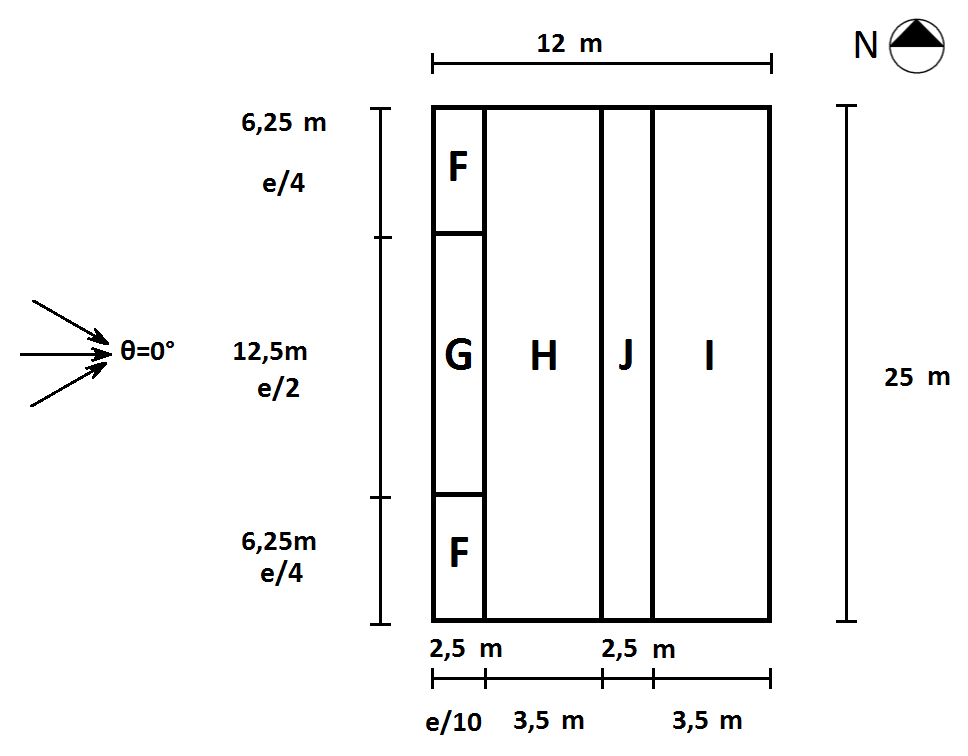
\includegraphics[width=0.8\textwidth]{billeder/opdeling.png}
	\caption{Opdeling af bygning, for vindretning fra øst og vest}
	\label{fig:opdeling}
\end{figure}

Formfaktoren, $c_{pe}$ kan bestemmes for taghældning på $26,\!56^{\circ}$, og der laves derfor lineær regression mellem $c_{pe}$ værdierne og graderne 15 og 30, efter anbefaling af det nationale anneks for alle $c_{pe}$ værdierne, som aflæses i \citep[ tabel 7.4a kapitel 7.2.5]{EU91}. For $\theta = 0^{\circ}$ skifter trykket hurtigt mellem positive og negative værdier i vindsiden, ved en taghældning mellem $\alpha = -5^{\circ} til + 45^{\circ}$, og derfor skal der regnes for både positive og negative formfaktorværdier. 
\newline \indent{     }  Nedenfor er et beregningseksempel for beregning af formfaktoren.
\newline
\newline
\underline{Zone F for vind fra vest}
\newline
Ud fra \citep[ tabel 7.4a kapitel 7.2.5]{EU91} er de negative værdier for zone F: $-0,\!9$ og $-0,\!5$. Her ud fra fås ligningen, og $c_{pe,10,neg}$ bestemmes:
\begin{center}
	$f(\alpha)=0,\!0267\alpha - 1,\!3 \to c_{pe,10,neg}=-0,\!592$
\end{center}
De positive værdier for zone F er: $0,\!2$ og $0,\!7$. Her ud fra fås ligningen, og $c_{pe,10,pos}$ bestemmes:
\begin{center}
	$f(\alpha)=0,\!0333\alpha - 0,\!3 \to c_{pe,10,pos}=0,\!585$
\end{center}

De beregnede værdier for formfaktoren ses i Tabellerne; \ref{tab:cc} og \ref{tab:kk}. 
\newline
\newline
De udvendige vindtryk beregnes ved formlen, som tidligere vist:
\begin{center} 
	$w_e=q_p(z_e)c_{pe}$
\end{center}

De indvendige vindtryk skal nu bestemmes, da de virker på samme tid som de udvendige vindtryk. For invendig vintryk er der tale om begreberne sug og træk.
\newline \indent{     }  Når vindtrykket, både ind- og udvendigt, har retning mod overfladen, er der tale om tryk, som regnes positivt. Ved negative tryk, med retning væk fra overfladen, er der tale om sug.
\newline
\newline
Den indre vindlast virker altid i samme retning på alle indre overflader. Der kan derfor kun være enten tryk eller sug, og aldirg begge dele på samme tid.
\newline
\newline
Der findes to måder til bestemmelse af formfaktoren, $c_{pi}$, for indvendig vind. I dette projekt anvendes den forsimplede metode, hvor $c_{pi}$ regnes til at være den mindst gunstige af + 0,2 og - 0,3 \citep[Kapitel 7]{EU91}. Værdierne for formfaktoren ses i Tabellerne \ref{tab:cc} og \ref{tab:kk}.
\newline
\newline
Herefter kan de indvendige vindtryk beregnes ved formlen, som tidligere vist:
\begin{center} 
	$w_e=q_p(z_e)c_{pi}$
\end{center}

\begin{table}[htb]
	\begin{center}
		\begin{tabular}{ |c|c|c|c|c| } 
			\hline
			Zone/Formfaktor & Positiv ud.& Negativ ud. & Positiv ind. & Negativ ind. \\	\hline
			F & 0,585 & -0,592 & 0,200 & -0,300 \\	\hline
			G & 0,585 & -0,569 & 0,200 & -0,300 \\	\hline 
			H & 0,354 & -0,223 & 0,200 & -0,300 \\ 	\hline
			I & 0 & -0,400 & 0,200 & -0,300 \\	\hline
			J & 0 & -0,615 & 0,200 & -0,300 \\	\hline
		\end{tabular}
		\caption{Værdier for $c_{pe,10}$ på udvendige og indvendige tagoverflader for vind fra vest og øst, vindretning $0^{\circ} = 180^{\circ}$ på taget}
		\label{tab:cc}
	\end{center}
\end{table}

\begin{table}[htb]
	\begin{center}
		\begin{tabular}{ |c|c|c|c| } 
			\hline
			Zone/Formfaktor & Negativ ud. & Positiv ind. & Negativ ind. \\	\hline
			F & -1,146 & 0,200 & -0,300 \\	\hline
			G & -1,377 & 0,200 & -0,300 \\	\hline 
			H & -0,754 & 0,200 & -0,300 \\ 	\hline
			I & -0,500 & 0,200 & -0,300 \\	\hline
		\end{tabular}
		\caption{Værdier for $c_{pe,10}$ på udvendige og indvendige tagoverflader for vind fra nord, vindretning $90^{\circ}$ på taget}
		\label{tab:kk}
	\end{center}
\end{table}

For at bestemme nettovindtrykket, som bestemmes ud fra formlen nedenfor, skal der opstilles en række tilfælde for, hvordan sug og tryk kan virke i samspil.
\newline
\newline
Der opstilles fire vindkombinationer for hver vindretning:
\begin{enumerate}
	\item Tryk udvendigt på FGH + sug for JI og invendigt sug
	\item Tryk udvendigt på FGH + sug for JI og invendigt tryk
	\item Sug udvendigt for FGH + tryk på JI og invendigt sug
	\item Sug udvendigt for FGH + tryk på JI og invendigt tryk
\end{enumerate}

Nedenfor laves et beregningseksempel med vind fra vest med vindkombination 1 zone F. De resternede værdier kan ses i Tabel \ref{tab:bb}.
\newline
\newline
Enheden skal være $[\frac{kN}{m}]$, og derfor ganges med længden mellem hver af vores stænger, som er 6,25 m.

\begin{center} 
	$w_F=(w_{e,F}-w_{i,F})\cdot 6,\!25 m$
\end{center}

\begin{itemize}
	\item[-] $w_{e,F}$: udvendig vindtryk for zone F
	\item[-] $w_{i,F}$: indvendig vindtryk for zone F
\end{itemize}

\begin{center} 
	$w_F=(q_{p,19 m}c_{e,pos. ud.}-q_{p,19 m}-c_{i,neg. ind.})\cdot 6,\!25 m = (0,\!579 \frac{kN}{m^2}\cdot 0,\!585 - 0,\!579 \frac{kN}{m^2}\cdot -0,\!300)\cdot 6,\!25 m = 3,\!203 \frac{kN}{m}$
\end{center}

For alle vindretningerne anvendes vindkombination 1 til videre beregning, hvor værdierne for indtryk på tagoverflader med tryk for udvendig vind fra vest og øst på F, G og H, og sug på I og J, mens der er sug fra nord på alle fire tagzoner og den indvendige vind er sug for alle.

\begin{table}[htb]
	\begin{center}
		\begin{tabular}{ |c|c|c|c| } 
			\hline
			Zone/Vindretning, w $[\frac{kN}{m}]$ & Vest & Øst & Nord \\	\hline
			F & 3,203 & 2,563 & -2,445 \\	\hline
			G & 3,203 & 2,563 & -3,804 \\	\hline 
			H & 2,367 & 1,893 & -1,314 \\ 	\hline
			I & -0,362 & -0,289 & -0,579 \\	\hline
			J & -1,138 & -0,910 & - \\	\hline
		\end{tabular}
		\caption{Værdier for nettovindtryk på taget}
		\label{tab:bb}
	\end{center}
\end{table}

Fra Tabel \ref{tab:bb} ses, at værdierne for vest er større i forhold til for øst, og formodentlig også mere kritiske. Vind fra nord kan kun påvirke taget med sug, og dermed ses der i denne raport bort fra denne. Derfor anvendes værdierne for vest til videre beregning i lastkombinationer, når der skal opstilles lastkombinationer for taget, og der ses fremover bort fra vind fra øst og nord på taget.
\newline
\newline
\underline{Vindtryk på facaderne}
\newline
Vinden vil også påvirke Strøybergs Palæ på dens facader og endegavle, og derfor skal vindlasten også beregnes for de lodrette vægge af bygningen.
\newline \indent{     }  Nettovindtrykket på facaderne beregnes som nettovindtrykket for taget, dog tages der udgangspunkt i \citep[ tabel 7.1]{EU91}. Her skal længden af bygningen anvendes, og igen bruges den fulde længde af bygningen, der består af den nuværende bygning og tilbygningen, som er 25 m. 
\newline
\newline
For vindretning $\Theta = 0^{\circ}$ for vind fra vest og øst gælder at b = 25 m, d = 12 m og højden h = 16 m på Figur \ref{fig:vindvest} og \ref{fig:vindost}. For vind fra nord gælder det at b = 25 m og h = 16 m.

\begin{figure}[htbp]
	\centering
	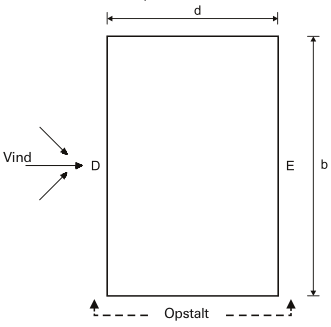
\includegraphics[width=0.5\textwidth]{billeder/vindvest1.png}
	\caption{Vind på facaden fra vest}
	\label{fig:vindvest}
\end{figure}

\begin{figure}[htbp]
	\centering
	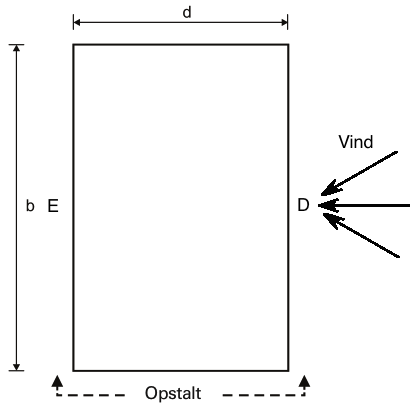
\includegraphics[width=0.5\textwidth]{billeder/vindost1.png}
	\caption{Vind på facaden fra øst}
	\label{fig:vindost}
\end{figure}

Bygningen deles op i zoner for vind fra vest og øst, som kan ses på Figur \ref{fig:ab}, mens den deles op i zoner for vind fra nord, der kan ses på Figur \ref{fig:ac}.

\begin{figure}[htbp]
	\centering
	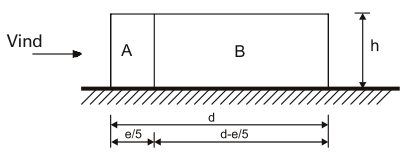
\includegraphics[width=0.7\textwidth]{billeder/vestost.png}
	\caption{Zoner for vind fra vest og øst på facaderne}
	\label{fig:ab}
\end{figure}

\begin{figure}[htbp]
	\centering
	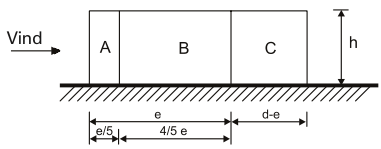
\includegraphics[width=0.7\textwidth]{billeder/nord.png}
	\caption{Zoner for vind fra nord på gavlen}
	\label{fig:ac}
\end{figure}

Ligesom for vind på tag opstilles der vindkombinationer for facaderne og gavlen:
\begin{enumerate}
	\item Tryk udvendigt på D og sug indvendigt
	\item Sug udvendigt på E og sug indvendigt
	\item Tryk udvendigt på D og tryk indvendigt  
	\item Sug udvendigt på E og tryk indvendigt
\end{enumerate}

Der arbejdes videre med vindkombination 1, hvor den udvendige vind virker som tryk på siden D og sug på siden E samt den indre vindlast er sug.
\newline \indent{     }  Værdierne for nettovindtrykket kan ses på Figur \ref{tab:hh}.

\begin{table}[htb]
	\begin{center}
		\begin{tabular}{ |c|c|c|c| } 
			\hline
			\multirow{2}{*}{Zone/Formfaktor} & \multirow{2}{*}{$c_{pe,10}$ udvendig} & \multicolumn{2}{l|}{$c_{pe,10}$ indvendig} \\ \cline{3-4} 
			& & Positiv & Negativ   		\\ \hline
			A & -1,200 & 0,200 & -0,300 \\	\hline
			B & -0,800 & 0,200 & -0,300 \\	\hline 
			D & 0,800 & 0,200 & -0,300 \\	\hline
			E & -0,517 & 0,200 & -0,300 \\	\hline
		\end{tabular}
		\caption{Værdier for $c_{pe,10}$ for vind fra vest og øst}
		\label{tab:ff}
	\end{center}
\end{table}

\begin{table}[htb]
	\begin{center}
		\begin{tabular}{ |c|c|c|c| } 
			\hline
			\multirow{2}{*}{Zone/Formfaktor} & \multirow{2}{*}{$c_{pe,10}$ udvendig} & \multicolumn{2}{l|}{$c_{pe,10}$ indvendig} \\ \cline{3-4} 
			& & Positiv & Negativ   		\\ \hline
			A & -1,200 & 0,200 & -0,300 \\	\hline
			B & -0,800 & 0,200 & -0,300 \\	\hline
			C & -0,500 & 0,200 & -0,300 \\	\hline 
			D & 0,752 & 0,200 & -0,300 \\	\hline
			E & -0,404 & 0,200 & -0,300 \\	\hline
		\end{tabular}
		\caption{Værdier for $c_{pe,10}$ for vind fra nord}
		\label{tab:gg}
	\end{center}
\end{table}

\begin{table}[htb]
	\begin{center}
		\begin{tabular}{|c|c|c|c|}
			\hline
			Zone/Vindretning, w $[\frac{kN}{m}]$ & Vest & Øst & Nord \\ \hline
			D & 3,686 & 2,946 & 2,142 \\ \hline
			E & -0,726 & -0,580 & -0,953 \\ \hline
		\end{tabular}
		\caption{Værdier for nettovindtryk på siderne}
		\label{tab:hh}
	\end{center}
\end{table}

Her ses, at værdierne for vest er størst, og formodentligt også mere kritiske. Derfor anvendes disse tal videre i lastkombinationer, når der skal opstilles lastkombinationer for taget, og igen ses der nu bort fra vind fra øst og nord for vind på siderne.
\newline \indent{     }  Disse linjelaster virker på højden af facaderne, der er siderne D og E, som hver er 16 m høje.
\newline
\newline
\underline{Opsummering}
\newline
Det er nu bestemt i denne rapport, at der fokuseres på vind fra vest, hvor der optræder forskellige udvendige laster, mens den indre altid optræder som sug. Lasterne er omregnet til linjelaster ved at gange med afstanden mellem vores rammer, hvilken er 6,25 m. 
\newline
\newline
Systemet betragtes, hvor der laves beregninger for rammen i midten af konstruktionen, hvilken ligger 6,25 m inde på konstruktionen. Det betyder, rammen ligger mellem zone F og G (se Figur \ref{fig:opdeling}). Derfor udregnes et gennemsnit mellem værdierne for zonerne F og G ved vind på taget, da zonen E for siderne gælder for hele facaden. 
Dog ses det, at værdierne F og G for taget er ens, og dermed er gennemsnitsværdien lig værdien for F og G. 

\subsection{Nyttelast}
Ud fra \citep[ tabel 6.2 kapitel 6.3.1.2]{EU91} aflæses den jævnt fordelte last, $q_k$, for kategori A1, som er bolig og lokale adgangsveje, til at være $1,\!5 \frac{kN}{m^2}$. Denne last beregnes for alle etager på tilbygningen samlet set.
\begin{center}
	$Q_{K3}=q_k A etageantal$
\end{center}
\begin{itemize}
	\item[-] A: arealet af én etage, som sættes til $150,\!0 m^2$
	\item[-] antal etager for tilbygningen er 5, men der ses bort fra kælderetagen
\end{itemize}
Nyttelasten kan nu bestemmes til:
\begin{center}
	$Q_{K3}=1,\!5 \frac{kN}{m^2}\cdot 150,\!0 m^2\cdot 4=900,\!0 kN$
\end{center}

\section{Lastkombinationer}
Den karakteristiske egenlast, jordlast, vindlast, snelast og nyttelast er bestemt for tilbygningen til Strøybergs Palæ. Derfor opstilles derfor en række forskellige lasttilfælde, for at beregne de regningsmæssige laster, som skal anvendes til beregningerne af reaktioskræfter for det statiske system af tilbygningen til Strøybergs Palæ.
\newline \indent{     }  Lastkombinationerne opstilles ved at betragte tilbygningen i tre dele; Taget, rammen mellem jorden og taget samt rammen under jorden. Disse deles ind i områder, da lasterne ikke virker ens på alle konstruktionsdele, hvilket er illustreret på Figur (INDSÆT FIGUR AF OMRÅDER PÅ STATISK SYSTEM).
\newline
\newline
Ved et rigtigt byggeprojekt skal der opstilles lasttilfælde for alle tænkelige scenarier, som kan forekomme. For dette projekt er det dog ikke en mulighed, og derfor fokuseres der kun udvalgte tilfælde.
\newline
\newline
Formlen for den regningsmæssige last er:
\begin{center}
	$E_d = \gamma_{G1} K_{FI} G_{K1} + \gamma_{Q1} K{FI} Q{K1} + \gamma_{Q2} \Psi_{0,2} K_{FI} Q_{K2} + \gamma_{Q3} \Psi_{0,3} K_{FI} Q_{K3}$ 
\end{center}

\begin{itemize}
	\item[-] $\gamma_G$: Partialkoefficient for permanent last
	\item[-] $K_{FI}$: Konsekvensklasse
	\item[-] $G_K$: Karakteristisk værdi for permanent last
	\item[-] $\gamma_Q$: Partialkoefficient for variabel last
	\item[-] $Q_K$: Karakteristisk værdi for variabel last
	\item[-] $\Psi$: Kombinationsværdi af variabel last. Mulitipliceres den værdi, som ikke er dominerende 
\end{itemize}

Der er lavet tre lasttilfælde for områder 1; for henholdsvis egenlasten, snelasten og vindlasten dominerende. Snelasten dominerende er beregnet ved: VENT MED AT INDSÆTTE TIL DET ER GODKENDT AF JOHAN. 
\newline
\newline
Nedenstående tabel viser resultaterne for hvert område, med skiftende dominerende laster.
\newline
\newline
INDSÆT TABEL MED VÆRDI FOR LASTTILFÆLDE!
\newline
\newline